\PassOptionsToPackage{unicode=true}{hyperref} % options for packages loaded elsewhere
\PassOptionsToPackage{hyphens}{url}
%
\documentclass[]{book}
\usepackage{lmodern}
\usepackage{amssymb,amsmath}
\usepackage{ifxetex,ifluatex}
\usepackage{fixltx2e} % provides \textsubscript
\ifnum 0\ifxetex 1\fi\ifluatex 1\fi=0 % if pdftex
  \usepackage[T1]{fontenc}
  \usepackage[utf8]{inputenc}
  \usepackage{textcomp} % provides euro and other symbols
\else % if luatex or xelatex
  \usepackage{unicode-math}
  \defaultfontfeatures{Ligatures=TeX,Scale=MatchLowercase}
\fi
% use upquote if available, for straight quotes in verbatim environments
\IfFileExists{upquote.sty}{\usepackage{upquote}}{}
% use microtype if available
\IfFileExists{microtype.sty}{%
\usepackage[]{microtype}
\UseMicrotypeSet[protrusion]{basicmath} % disable protrusion for tt fonts
}{}
\IfFileExists{parskip.sty}{%
\usepackage{parskip}
}{% else
\setlength{\parindent}{0pt}
\setlength{\parskip}{6pt plus 2pt minus 1pt}
}
\usepackage{hyperref}
\hypersetup{
            pdftitle={Diagnostics Supplemental Material},
            pdfauthor={Jose Guadalupe Hernandez},
            pdfborder={0 0 0},
            breaklinks=true}
\urlstyle{same}  % don't use monospace font for urls
\usepackage{color}
\usepackage{fancyvrb}
\newcommand{\VerbBar}{|}
\newcommand{\VERB}{\Verb[commandchars=\\\{\}]}
\DefineVerbatimEnvironment{Highlighting}{Verbatim}{commandchars=\\\{\}}
% Add ',fontsize=\small' for more characters per line
\usepackage{framed}
\definecolor{shadecolor}{RGB}{248,248,248}
\newenvironment{Shaded}{\begin{snugshade}}{\end{snugshade}}
\newcommand{\AlertTok}[1]{\textcolor[rgb]{0.94,0.16,0.16}{#1}}
\newcommand{\AnnotationTok}[1]{\textcolor[rgb]{0.56,0.35,0.01}{\textbf{\textit{#1}}}}
\newcommand{\AttributeTok}[1]{\textcolor[rgb]{0.77,0.63,0.00}{#1}}
\newcommand{\BaseNTok}[1]{\textcolor[rgb]{0.00,0.00,0.81}{#1}}
\newcommand{\BuiltInTok}[1]{#1}
\newcommand{\CharTok}[1]{\textcolor[rgb]{0.31,0.60,0.02}{#1}}
\newcommand{\CommentTok}[1]{\textcolor[rgb]{0.56,0.35,0.01}{\textit{#1}}}
\newcommand{\CommentVarTok}[1]{\textcolor[rgb]{0.56,0.35,0.01}{\textbf{\textit{#1}}}}
\newcommand{\ConstantTok}[1]{\textcolor[rgb]{0.00,0.00,0.00}{#1}}
\newcommand{\ControlFlowTok}[1]{\textcolor[rgb]{0.13,0.29,0.53}{\textbf{#1}}}
\newcommand{\DataTypeTok}[1]{\textcolor[rgb]{0.13,0.29,0.53}{#1}}
\newcommand{\DecValTok}[1]{\textcolor[rgb]{0.00,0.00,0.81}{#1}}
\newcommand{\DocumentationTok}[1]{\textcolor[rgb]{0.56,0.35,0.01}{\textbf{\textit{#1}}}}
\newcommand{\ErrorTok}[1]{\textcolor[rgb]{0.64,0.00,0.00}{\textbf{#1}}}
\newcommand{\ExtensionTok}[1]{#1}
\newcommand{\FloatTok}[1]{\textcolor[rgb]{0.00,0.00,0.81}{#1}}
\newcommand{\FunctionTok}[1]{\textcolor[rgb]{0.00,0.00,0.00}{#1}}
\newcommand{\ImportTok}[1]{#1}
\newcommand{\InformationTok}[1]{\textcolor[rgb]{0.56,0.35,0.01}{\textbf{\textit{#1}}}}
\newcommand{\KeywordTok}[1]{\textcolor[rgb]{0.13,0.29,0.53}{\textbf{#1}}}
\newcommand{\NormalTok}[1]{#1}
\newcommand{\OperatorTok}[1]{\textcolor[rgb]{0.81,0.36,0.00}{\textbf{#1}}}
\newcommand{\OtherTok}[1]{\textcolor[rgb]{0.56,0.35,0.01}{#1}}
\newcommand{\PreprocessorTok}[1]{\textcolor[rgb]{0.56,0.35,0.01}{\textit{#1}}}
\newcommand{\RegionMarkerTok}[1]{#1}
\newcommand{\SpecialCharTok}[1]{\textcolor[rgb]{0.00,0.00,0.00}{#1}}
\newcommand{\SpecialStringTok}[1]{\textcolor[rgb]{0.31,0.60,0.02}{#1}}
\newcommand{\StringTok}[1]{\textcolor[rgb]{0.31,0.60,0.02}{#1}}
\newcommand{\VariableTok}[1]{\textcolor[rgb]{0.00,0.00,0.00}{#1}}
\newcommand{\VerbatimStringTok}[1]{\textcolor[rgb]{0.31,0.60,0.02}{#1}}
\newcommand{\WarningTok}[1]{\textcolor[rgb]{0.56,0.35,0.01}{\textbf{\textit{#1}}}}
\usepackage{longtable,booktabs}
% Fix footnotes in tables (requires footnote package)
\IfFileExists{footnote.sty}{\usepackage{footnote}\makesavenoteenv{longtable}}{}
\usepackage{graphicx,grffile}
\makeatletter
\def\maxwidth{\ifdim\Gin@nat@width>\linewidth\linewidth\else\Gin@nat@width\fi}
\def\maxheight{\ifdim\Gin@nat@height>\textheight\textheight\else\Gin@nat@height\fi}
\makeatother
% Scale images if necessary, so that they will not overflow the page
% margins by default, and it is still possible to overwrite the defaults
% using explicit options in \includegraphics[width, height, ...]{}
\setkeys{Gin}{width=\maxwidth,height=\maxheight,keepaspectratio}
\setlength{\emergencystretch}{3em}  % prevent overfull lines
\providecommand{\tightlist}{%
  \setlength{\itemsep}{0pt}\setlength{\parskip}{0pt}}
\setcounter{secnumdepth}{5}
% Redefines (sub)paragraphs to behave more like sections
\ifx\paragraph\undefined\else
\let\oldparagraph\paragraph
\renewcommand{\paragraph}[1]{\oldparagraph{#1}\mbox{}}
\fi
\ifx\subparagraph\undefined\else
\let\oldsubparagraph\subparagraph
\renewcommand{\subparagraph}[1]{\oldsubparagraph{#1}\mbox{}}
\fi

% set default figure placement to htbp
\makeatletter
\def\fps@figure{htbp}
\makeatother

\usepackage[]{natbib}
\bibliographystyle{apalike}

\title{Diagnostics Supplemental Material}
\author{Jose Guadalupe Hernandez}
\date{2022-11-22}

\begin{document}
\maketitle

{
\setcounter{tocdepth}{1}
\tableofcontents
}
\hypertarget{introduction}{%
\chapter{Introduction}\label{introduction}}

This is the supplemental material associated with our 2022 ECJ contribution entitled, \emph{A suite of diagnostic metrics for characterizing selection schemes}.
Preprint \href{https://arxiv.org/pdf/2204.13839.pdf}{here}.

\hypertarget{about-our-supplemental-material}{%
\section{About our supplemental material}\label{about-our-supplemental-material}}

This supplemental material is hosted on \href{https://github.com}{GitHub} using GitHub pages.
The source code and configuration files used to generate this supplemental material can be found in \href{https://github.com/jgh9094/ECJ-2022-suite-of-diagnostics-for-selection-schemes}{this GitHub repository}.
We compiled our data analyses and supplemental documentation into this nifty web-accessible book using \href{https://bookdown.org/}{bookdown}.

Our supplemental material includes the following paper figures and statistics:

\begin{itemize}
\tightlist
\item
  Exploitation rate results (Section \ref{exploitation-rate-results})
\item
  Ordered exploitation results (Section \ref{ordered-exploitation-results})
\item
  Contradictory objectives results (Section \ref{contradictory-objectives-results})
\item
  Multi-path exploration results (Section \ref{multi-path-exploration-results})
\item
  Multi-valley crossing results (Section \ref{multi-valley-crossing-results})
\end{itemize}

Additionally, our supplemental material includes the results from parameter tuning selection schemes:

\begin{itemize}
\tightlist
\item
  Truncation selection (Section \ref{truncation-selection})
\item
  Tournament selection sharing (Section \ref{tournament-selection})
\item
  Genotypic fitness sharing (Section \ref{genotypic-fitness-sharing})
\item
  Phenotypic fitness sharing (Section \ref{phenotypic-fitness-sharing})
\item
  Nondominated sorting (Section \ref{nondominated-sorting})
\item
  Novelty search (Section \ref{novelty-search})
\end{itemize}

\hypertarget{contributing-authors}{%
\section{Contributing authors}\label{contributing-authors}}

\begin{itemize}
\tightlist
\item
  \href{https://jgh9094.github.io/}{Jose Guadalupe Hernandez}
\item
  \href{https://lalejini.com}{Alexander Lalejini}
\item
  \href{http://ofria.com}{Charles Ofria}
\end{itemize}

\hypertarget{research-overview}{%
\section{Research overview}\label{research-overview}}

\textbf{Abstract}:

Evolutionary algorithms typically consist of multiple interacting components, where each component influences an algorithm's problem-solving abilities.
Understanding how each component of an evolutionary algorithm influences problem-solving success can improve our ability to target particular problem domains.
Benchmark suites provide insights into an evolutionary algorithm's problem-solving capabilities, but benchmarking problems often have complex search space topologies, making it difficult to isolate and test an algorithm's strengths and weaknesses.
Our work focuses on diagnosing selection schemes, which identify individuals to contribute genetic material to the next generation, thus driving an evolutionary algorithm's search strategy.
We introduce four diagnostics for empirically testing the strengths and weaknesses of selection schemes: the exploitation rate diagnostic, ordered exploitation rate diagnostic, contradictory objectives diagnostic, and the multi-path exploration diagnostic.
Each diagnostic is a handcrafted search space designed to isolate and measure the relative exploitation and exploration characteristics of selection schemes.
Here, we use our diagnostics to evaluate six population selection methods: truncation selection, tournament selection, fitness sharing, lexicase selection, nondominated sorting, and novelty search.
Expectedly, tournament and truncation selection excelled at gradient exploitation but poorly explored search spaces, while novelty search excelled at exploration but failed to exploit gradients.
Fitness sharing performed poorly across all diagnostics, suggesting poor overall exploitation and exploration abilities.
Nondominated sorting was best for maintaining diverse populations comprised of individuals inhabiting multiple optima, but struggled to effectively exploit gradients.
Lexicase selection balanced search space exploration without sacrificing exploitation, generally performing well across diagnostics.
Our work demonstrates the value of diagnostics for building a deeper understanding of selection schemes, which can then be used to improve or develop new selection methods.

\hypertarget{experimental-setup}{%
\section{Experimental setup}\label{experimental-setup}}

Setting up required variables variables.

\begin{Shaded}
\begin{Highlighting}[]
\KeywordTok{library}\NormalTok{(ggplot2)}
\KeywordTok{library}\NormalTok{(dplyr)}
\end{Highlighting}
\end{Shaded}

\begin{verbatim}
## 
## Attaching package: 'dplyr'
\end{verbatim}

\begin{verbatim}
## The following objects are masked from 'package:stats':
## 
##     filter, lag
\end{verbatim}

\begin{verbatim}
## The following objects are masked from 'package:base':
## 
##     intersect, setdiff, setequal, union
\end{verbatim}

\begin{Shaded}
\begin{Highlighting}[]
\CommentTok{# variables used throughout}
\NormalTok{TRAITS =}\StringTok{ }\DecValTok{100}
\NormalTok{TSIZE =}\StringTok{ }\DecValTok{26}
\NormalTok{ORDER =}\StringTok{ }\KeywordTok{c}\NormalTok{(}\StringTok{'Truncation (tru)'}\NormalTok{,}\StringTok{'Tournament (tor)'}\NormalTok{,}\StringTok{'Lexicase (lex)'}\NormalTok{, }\StringTok{'Genotypic Fitness Sharing (gfs)'}\NormalTok{,}\StringTok{'Phenotypic Fitness Sharing (pfs)'}\NormalTok{,}\StringTok{'Nondominated Sorting (nds)'}\NormalTok{,}\StringTok{'Novelty Search (nov)'}\NormalTok{,}\StringTok{'Random (ran)'}\NormalTok{)}
\NormalTok{ACRON =}\StringTok{ }\KeywordTok{tolower}\NormalTok{(}\KeywordTok{c}\NormalTok{(}\StringTok{'TRU'}\NormalTok{,}\StringTok{'TOR'}\NormalTok{,}\StringTok{'LEX'}\NormalTok{,}\StringTok{'GFS'}\NormalTok{,}\StringTok{'PFS'}\NormalTok{,}\StringTok{'NDS'}\NormalTok{,}\StringTok{'NOV'}\NormalTok{,}\StringTok{'RAN'}\NormalTok{))}
\NormalTok{SHAPE =}\StringTok{ }\KeywordTok{c}\NormalTok{(}\DecValTok{5}\NormalTok{,}\DecValTok{3}\NormalTok{,}\DecValTok{1}\NormalTok{,}\DecValTok{2}\NormalTok{,}\DecValTok{6}\NormalTok{,}\DecValTok{0}\NormalTok{,}\DecValTok{4}\NormalTok{,}\DecValTok{20}\NormalTok{,}\DecValTok{1}\NormalTok{)}
\NormalTok{PARAM =}\StringTok{ }\KeywordTok{c}\NormalTok{(}\StringTok{'8'}\NormalTok{, }\StringTok{'8'}\NormalTok{, }\StringTok{'0.0'}\NormalTok{, }\StringTok{'0.3'}\NormalTok{, }\StringTok{'0.3'}\NormalTok{, }\StringTok{'0.3'}\NormalTok{, }\StringTok{'15'}\NormalTok{, }\StringTok{'1'}\NormalTok{)}
\NormalTok{cb_palette <-}\StringTok{ }\KeywordTok{c}\NormalTok{(}\StringTok{'#332288'}\NormalTok{,}\StringTok{'#88CCEE'}\NormalTok{,}\StringTok{'#EE7733'}\NormalTok{,}\StringTok{'#EE3377'}\NormalTok{,}\StringTok{'#117733'}\NormalTok{,}\StringTok{'#882255'}\NormalTok{,}\StringTok{'#44AA99'}\NormalTok{,}\StringTok{'#CCBB44'}\NormalTok{, }\StringTok{'#000000'}\NormalTok{)}
\NormalTok{GENERATIONS =}\StringTok{ }\DecValTok{50000}

\CommentTok{# selection scheme parameters}
\NormalTok{TR_LIST =}\StringTok{ }\KeywordTok{c}\NormalTok{(}\DecValTok{1}\NormalTok{, }\DecValTok{2}\NormalTok{, }\DecValTok{4}\NormalTok{, }\DecValTok{8}\NormalTok{, }\DecValTok{16}\NormalTok{, }\DecValTok{32}\NormalTok{, }\DecValTok{64}\NormalTok{, }\DecValTok{128}\NormalTok{, }\DecValTok{256}\NormalTok{)}
\NormalTok{TS_LIST =}\StringTok{ }\KeywordTok{c}\NormalTok{(}\DecValTok{2}\NormalTok{, }\DecValTok{4}\NormalTok{, }\DecValTok{8}\NormalTok{, }\DecValTok{16}\NormalTok{, }\DecValTok{32}\NormalTok{, }\DecValTok{64}\NormalTok{, }\DecValTok{128}\NormalTok{, }\DecValTok{256}\NormalTok{)}
\NormalTok{FS_LIST =}\StringTok{ }\KeywordTok{c}\NormalTok{(}\FloatTok{0.0}\NormalTok{, }\FloatTok{0.1}\NormalTok{, }\FloatTok{0.3}\NormalTok{, }\FloatTok{0.6}\NormalTok{, }\FloatTok{1.2}\NormalTok{, }\FloatTok{2.5}\NormalTok{, }\FloatTok{5.0}\NormalTok{)}
\NormalTok{ND_LIST =}\StringTok{ }\KeywordTok{c}\NormalTok{(}\FloatTok{0.0}\NormalTok{, }\FloatTok{0.1}\NormalTok{, }\FloatTok{0.3}\NormalTok{, }\FloatTok{0.6}\NormalTok{, }\FloatTok{1.2}\NormalTok{, }\FloatTok{2.5}\NormalTok{, }\FloatTok{5.0}\NormalTok{)}
\NormalTok{NS_LIST =}\StringTok{ }\KeywordTok{c}\NormalTok{(}\DecValTok{1}\NormalTok{, }\DecValTok{2}\NormalTok{, }\DecValTok{4}\NormalTok{, }\DecValTok{8}\NormalTok{, }\DecValTok{15}\NormalTok{, }\DecValTok{30}\NormalTok{)}

\CommentTok{# theme that graphs will follow}
\NormalTok{p_theme <-}\StringTok{ }\KeywordTok{theme}\NormalTok{(}
  \DataTypeTok{text =} \KeywordTok{element_text}\NormalTok{(}\DataTypeTok{size =} \DecValTok{28}\NormalTok{),}
  \DataTypeTok{plot.title =} \KeywordTok{element_text}\NormalTok{( }\DataTypeTok{face =} \StringTok{"bold"}\NormalTok{, }\DataTypeTok{size =} \DecValTok{22}\NormalTok{, }\DataTypeTok{hjust=}\FloatTok{0.5}\NormalTok{),}
  \DataTypeTok{panel.border =} \KeywordTok{element_blank}\NormalTok{(),}
  \DataTypeTok{panel.grid.minor =} \KeywordTok{element_blank}\NormalTok{(),}
  \DataTypeTok{legend.title=}\KeywordTok{element_text}\NormalTok{(}\DataTypeTok{size=}\DecValTok{18}\NormalTok{),}
  \DataTypeTok{legend.text=}\KeywordTok{element_text}\NormalTok{(}\DataTypeTok{size=}\DecValTok{14}\NormalTok{),}
  \DataTypeTok{axis.title =} \KeywordTok{element_text}\NormalTok{(}\DataTypeTok{size=}\DecValTok{18}\NormalTok{),}
  \DataTypeTok{axis.text =} \KeywordTok{element_text}\NormalTok{(}\DataTypeTok{size=}\DecValTok{16}\NormalTok{),}
  \DataTypeTok{legend.position=}\StringTok{"bottom"}\NormalTok{,}
  \DataTypeTok{panel.background =} \KeywordTok{element_rect}\NormalTok{(}\DataTypeTok{fill =} \StringTok{"#f1f2f5"}\NormalTok{,}
                                  \DataTypeTok{colour =} \StringTok{"white"}\NormalTok{,}
                                  \DataTypeTok{size =} \FloatTok{0.5}\NormalTok{, }\DataTypeTok{linetype =} \StringTok{"solid"}\NormalTok{)}
\NormalTok{)}
\end{Highlighting}
\end{Shaded}

\begin{verbatim}
## Warning: The `size` argument of `element_rect()` is deprecated as of ggplot2 3.4.0.
## i Please use the `linewidth` argument instead.
\end{verbatim}

\begin{Shaded}
\begin{Highlighting}[]
\CommentTok{# cross comparison data frames}
\NormalTok{cc_over_time <-}\StringTok{ }\KeywordTok{read.csv}\NormalTok{(}\StringTok{'/opt/ECJ-2022-suite-of-diagnostics-for-selection-schemes/DATA-FINAL/POLISHED/cross-comp-over-time.csv'}\NormalTok{, }\DataTypeTok{header =} \OtherTok{TRUE}\NormalTok{, }\DataTypeTok{stringsAsFactors =} \OtherTok{FALSE}\NormalTok{)}
\KeywordTok{colnames}\NormalTok{(cc_over_time)[}\KeywordTok{colnames}\NormalTok{(cc_over_time) }\OperatorTok{==}\StringTok{ "Selection.Scheme"}\NormalTok{] =}\StringTok{ 'Selection}\CharTok{\textbackslash{}n}\StringTok{Scheme'}
\NormalTok{cc_over_time}\OperatorTok{$}\StringTok{`}\DataTypeTok{Selection}\CharTok{\textbackslash{}n}\DataTypeTok{Scheme}\StringTok{`}\NormalTok{ <-}\StringTok{ }\KeywordTok{factor}\NormalTok{(cc_over_time}\OperatorTok{$}\StringTok{`}\DataTypeTok{Selection}\CharTok{\textbackslash{}n}\DataTypeTok{Scheme}\StringTok{`}\NormalTok{, }\DataTypeTok{levels =}\NormalTok{ ORDER)}
\NormalTok{cc_over_time}\OperatorTok{$}\NormalTok{uni_str_pos =}\StringTok{ }\NormalTok{cc_over_time}\OperatorTok{$}\NormalTok{uni_str_pos }\OperatorTok{+}\StringTok{ }\NormalTok{cc_over_time}\OperatorTok{$}\NormalTok{arc_acti_gene }\OperatorTok{-}\StringTok{ }\NormalTok{cc_over_time}\OperatorTok{$}\NormalTok{overlap}

\NormalTok{cc_best =}\StringTok{ }\KeywordTok{read.csv}\NormalTok{(}\StringTok{'/opt/ECJ-2022-suite-of-diagnostics-for-selection-schemes/DATA-FINAL/POLISHED/cross-comp-best.csv'}\NormalTok{, }\DataTypeTok{header =} \OtherTok{TRUE}\NormalTok{, }\DataTypeTok{stringsAsFactors =} \OtherTok{FALSE}\NormalTok{)}
\NormalTok{cc_best}\OperatorTok{$}\NormalTok{acron <-}\StringTok{ }\KeywordTok{factor}\NormalTok{(cc_best}\OperatorTok{$}\NormalTok{acron, }\DataTypeTok{levels =}\NormalTok{ ACRON)}
\KeywordTok{colnames}\NormalTok{(cc_best)[}\KeywordTok{colnames}\NormalTok{(cc_best) }\OperatorTok{==}\StringTok{ "Selection.Scheme"}\NormalTok{] =}\StringTok{ 'Selection}\CharTok{\textbackslash{}n}\StringTok{Scheme'}

\NormalTok{cc_ssf =}\StringTok{ }\KeywordTok{read.csv}\NormalTok{(}\StringTok{'/opt/ECJ-2022-suite-of-diagnostics-for-selection-schemes/DATA-FINAL/POLISHED/selection-scheme-ssf.csv'}\NormalTok{, }\DataTypeTok{header =} \OtherTok{TRUE}\NormalTok{, }\DataTypeTok{stringsAsFactors =} \OtherTok{FALSE}\NormalTok{)}
\NormalTok{cc_ssf}\OperatorTok{$}\NormalTok{acron <-}\StringTok{ }\KeywordTok{factor}\NormalTok{(cc_ssf}\OperatorTok{$}\NormalTok{acron, }\DataTypeTok{levels =}\NormalTok{ ACRON)}
\KeywordTok{colnames}\NormalTok{(cc_over_time)[}\KeywordTok{colnames}\NormalTok{(cc_over_time) }\OperatorTok{==}\StringTok{ "Selection.Scheme"}\NormalTok{] =}\StringTok{ 'Selection}\CharTok{\textbackslash{}n}\StringTok{Scheme'}
\NormalTok{cc_ssf[}\KeywordTok{is.na}\NormalTok{(cc_ssf)] <-}\StringTok{ }\DecValTok{59999}

\NormalTok{cc_end <-}\StringTok{ }\KeywordTok{filter}\NormalTok{(cc_over_time, gen }\OperatorTok{==}\StringTok{ }\DecValTok{50000}\NormalTok{)}
\NormalTok{cc_end}\OperatorTok{$}\NormalTok{acron <-}\StringTok{ }\KeywordTok{factor}\NormalTok{(cc_end}\OperatorTok{$}\NormalTok{acron, }\DataTypeTok{levels =}\NormalTok{ ACRON)}

\CommentTok{# selection scheme data frames}
\NormalTok{ss_over_time <-}\StringTok{ }\KeywordTok{read.csv}\NormalTok{(}\StringTok{'/opt/ECJ-2022-suite-of-diagnostics-for-selection-schemes/DATA-FINAL/POLISHED/selection-scheme-over-time.csv'}\NormalTok{, }\DataTypeTok{header =} \OtherTok{TRUE}\NormalTok{, }\DataTypeTok{stringsAsFactors =} \OtherTok{FALSE}\NormalTok{)}
\KeywordTok{colnames}\NormalTok{(ss_over_time)[}\KeywordTok{colnames}\NormalTok{(ss_over_time) }\OperatorTok{==}\StringTok{ "Selection.Scheme"}\NormalTok{] =}\StringTok{ 'Selection}\CharTok{\textbackslash{}n}\StringTok{Scheme'}
\NormalTok{ss_over_time}\OperatorTok{$}\NormalTok{uni_str_pos =}\StringTok{ }\NormalTok{ss_over_time}\OperatorTok{$}\NormalTok{uni_str_pos }\OperatorTok{+}\StringTok{ }\NormalTok{ss_over_time}\OperatorTok{$}\NormalTok{arc_acti_gene }\OperatorTok{-}\StringTok{ }\NormalTok{ss_over_time}\OperatorTok{$}\NormalTok{overlap}

\NormalTok{ss_best <-}\StringTok{ }\KeywordTok{read.csv}\NormalTok{(}\StringTok{'/opt/ECJ-2022-suite-of-diagnostics-for-selection-schemes/DATA-FINAL/POLISHED/selection-scheme-best.csv'}\NormalTok{, }\DataTypeTok{header =} \OtherTok{TRUE}\NormalTok{, }\DataTypeTok{stringsAsFactors =} \OtherTok{FALSE}\NormalTok{)}
\KeywordTok{colnames}\NormalTok{(ss_best)[}\KeywordTok{colnames}\NormalTok{(ss_best) }\OperatorTok{==}\StringTok{ "Selection.Scheme"}\NormalTok{] =}\StringTok{ 'Selection}\CharTok{\textbackslash{}n}\StringTok{Scheme'}

\NormalTok{ss_ssf <-}\StringTok{ }\KeywordTok{read.csv}\NormalTok{(}\StringTok{'/opt/ECJ-2022-suite-of-diagnostics-for-selection-schemes/DATA-FINAL/POLISHED/selection-scheme-ssf.csv'}\NormalTok{, }\DataTypeTok{header =} \OtherTok{TRUE}\NormalTok{, }\DataTypeTok{stringsAsFactors =} \OtherTok{FALSE}\NormalTok{)}
\KeywordTok{colnames}\NormalTok{(ss_ssf)[}\KeywordTok{colnames}\NormalTok{(ss_ssf) }\OperatorTok{==}\StringTok{ "Selection.Scheme"}\NormalTok{] =}\StringTok{ 'Selection}\CharTok{\textbackslash{}n}\StringTok{Scheme'}

\CommentTok{## genotypic fitness sharing data frames}
\NormalTok{gfs_ot <-}\StringTok{ }\KeywordTok{filter}\NormalTok{(ss_over_time, acron }\OperatorTok{==}\StringTok{ 'gfs'}\NormalTok{)}
\NormalTok{gfs_ot}\OperatorTok{$}\NormalTok{Sigma <-}\StringTok{ }\KeywordTok{factor}\NormalTok{(gfs_ot}\OperatorTok{$}\NormalTok{trt, }\DataTypeTok{levels =}\NormalTok{ FS_LIST)}
\NormalTok{gfs_best <-}\StringTok{ }\KeywordTok{filter}\NormalTok{(ss_best, acron }\OperatorTok{==}\StringTok{ 'gfs'}\NormalTok{)}
\NormalTok{gfs_best}\OperatorTok{$}\NormalTok{Sigma <-}\StringTok{ }\KeywordTok{factor}\NormalTok{(gfs_best}\OperatorTok{$}\NormalTok{trt, }\DataTypeTok{levels =}\NormalTok{ FS_LIST)}
\NormalTok{gfs_end  <-}\StringTok{ }\KeywordTok{filter}\NormalTok{(gfs_ot, gen }\OperatorTok{==}\StringTok{ }\DecValTok{50000}\NormalTok{)}

\CommentTok{## phenotypic fitness sharing data frames}
\NormalTok{pfs_ot <-}\StringTok{ }\KeywordTok{filter}\NormalTok{(ss_over_time, acron }\OperatorTok{==}\StringTok{ 'pfs'}\NormalTok{)}
\NormalTok{pfs_ot}\OperatorTok{$}\NormalTok{Sigma <-}\StringTok{ }\KeywordTok{factor}\NormalTok{(pfs_ot}\OperatorTok{$}\NormalTok{trt, }\DataTypeTok{levels =}\NormalTok{ FS_LIST)}
\NormalTok{pfs_best <-}\StringTok{ }\KeywordTok{filter}\NormalTok{(ss_best, acron }\OperatorTok{==}\StringTok{ 'pfs'}\NormalTok{)}
\NormalTok{pfs_best}\OperatorTok{$}\NormalTok{Sigma <-}\StringTok{ }\KeywordTok{factor}\NormalTok{(pfs_best}\OperatorTok{$}\NormalTok{trt, }\DataTypeTok{levels =}\NormalTok{ FS_LIST)}
\NormalTok{pfs_end  <-}\StringTok{ }\KeywordTok{filter}\NormalTok{(pfs_ot, gen }\OperatorTok{==}\StringTok{ }\DecValTok{50000}\NormalTok{)}

\CommentTok{## nodominated sorting data frames}
\NormalTok{nds_ot <-}\StringTok{ }\KeywordTok{filter}\NormalTok{(ss_over_time, acron }\OperatorTok{==}\StringTok{ 'nds'}\NormalTok{)}
\NormalTok{nds_ot}\OperatorTok{$}\NormalTok{Sigma <-}\StringTok{ }\KeywordTok{factor}\NormalTok{(nds_ot}\OperatorTok{$}\NormalTok{trt, }\DataTypeTok{levels =}\NormalTok{ ND_LIST)}
\NormalTok{nds_best <-}\StringTok{ }\KeywordTok{filter}\NormalTok{(ss_best, acron }\OperatorTok{==}\StringTok{ 'nds'}\NormalTok{)}
\NormalTok{nds_best}\OperatorTok{$}\NormalTok{Sigma <-}\StringTok{ }\KeywordTok{factor}\NormalTok{(nds_best}\OperatorTok{$}\NormalTok{trt, }\DataTypeTok{levels =}\NormalTok{ ND_LIST)}
\NormalTok{nds_end  <-}\StringTok{ }\KeywordTok{filter}\NormalTok{(nds_ot, gen }\OperatorTok{==}\StringTok{ }\DecValTok{50000}\NormalTok{)}

\CommentTok{## novelty search data frames}
\NormalTok{nov_ot <-}\StringTok{ }\KeywordTok{filter}\NormalTok{(ss_over_time, acron }\OperatorTok{==}\StringTok{ 'nov'} \OperatorTok{&}\StringTok{ }\NormalTok{trt }\OperatorTok{!=}\StringTok{ }\DecValTok{0}\NormalTok{)}
\NormalTok{nov_ot}\OperatorTok{$}\NormalTok{K <-}\StringTok{ }\KeywordTok{factor}\NormalTok{(nov_ot}\OperatorTok{$}\NormalTok{trt, }\DataTypeTok{levels =}\NormalTok{ NS_LIST)}
\NormalTok{nov_best <-}\StringTok{ }\KeywordTok{filter}\NormalTok{(ss_best, acron }\OperatorTok{==}\StringTok{ 'nov'} \OperatorTok{&}\StringTok{ }\NormalTok{trt }\OperatorTok{!=}\StringTok{ }\DecValTok{0}\NormalTok{)}
\NormalTok{nov_best}\OperatorTok{$}\NormalTok{K <-}\StringTok{ }\KeywordTok{factor}\NormalTok{(nov_best}\OperatorTok{$}\NormalTok{trt, }\DataTypeTok{levels =}\NormalTok{ NS_LIST)}
\NormalTok{nov_end  <-}\StringTok{ }\KeywordTok{filter}\NormalTok{(nov_ot, gen }\OperatorTok{==}\StringTok{ }\DecValTok{50000}\NormalTok{)}

\CommentTok{## tournament data frames}
\NormalTok{tor_ot <-}\StringTok{ }\KeywordTok{filter}\NormalTok{(ss_over_time, acron }\OperatorTok{==}\StringTok{ 'tor'} \OperatorTok{&}\StringTok{ }\NormalTok{trt }\OperatorTok{!=}\StringTok{ }\DecValTok{1}\NormalTok{)}
\NormalTok{tor_ot}\OperatorTok{$}\NormalTok{T <-}\StringTok{ }\KeywordTok{factor}\NormalTok{(tor_ot}\OperatorTok{$}\NormalTok{trt, }\DataTypeTok{levels =}\NormalTok{ TS_LIST)}
\NormalTok{tor_best <-}\StringTok{ }\KeywordTok{filter}\NormalTok{(ss_best, acron }\OperatorTok{==}\StringTok{ 'tor'} \OperatorTok{&}\StringTok{ }\NormalTok{trt }\OperatorTok{!=}\StringTok{ }\DecValTok{1}\NormalTok{)}
\NormalTok{tor_best}\OperatorTok{$}\NormalTok{T <-}\StringTok{ }\KeywordTok{factor}\NormalTok{(tor_best}\OperatorTok{$}\NormalTok{trt, }\DataTypeTok{levels =}\NormalTok{ TS_LIST)}
\NormalTok{tor_end  <-}\StringTok{ }\KeywordTok{filter}\NormalTok{(tor_ot, gen }\OperatorTok{==}\StringTok{ }\DecValTok{50000}\NormalTok{)}
\NormalTok{tor_ssf <-}\StringTok{ }\KeywordTok{filter}\NormalTok{(ss_ssf, acron }\OperatorTok{==}\StringTok{ 'tor'} \OperatorTok{&}\StringTok{ }\NormalTok{trt }\OperatorTok{!=}\StringTok{ }\DecValTok{1}\NormalTok{)}
\NormalTok{tor_ssf}\OperatorTok{$}\NormalTok{T <-}\StringTok{ }\KeywordTok{factor}\NormalTok{(tor_ssf}\OperatorTok{$}\NormalTok{trt, }\DataTypeTok{levels =}\NormalTok{ TS_LIST)}
\NormalTok{tor_ssf[}\KeywordTok{is.na}\NormalTok{(tor_ssf)] <-}\StringTok{ }\DecValTok{59999}

\CommentTok{## truncation data frames}
\NormalTok{tru_ot <-}\StringTok{ }\KeywordTok{filter}\NormalTok{(ss_over_time, acron }\OperatorTok{==}\StringTok{ 'tru'}\NormalTok{)}
\NormalTok{tru_ot}\OperatorTok{$}\NormalTok{T <-}\StringTok{ }\KeywordTok{factor}\NormalTok{(tru_ot}\OperatorTok{$}\NormalTok{trt, }\DataTypeTok{levels =}\NormalTok{ TR_LIST)}
\NormalTok{tru_best <-}\StringTok{ }\KeywordTok{filter}\NormalTok{(ss_best, acron }\OperatorTok{==}\StringTok{ 'tru'}\NormalTok{)}
\NormalTok{tru_best}\OperatorTok{$}\NormalTok{T <-}\StringTok{ }\KeywordTok{factor}\NormalTok{(tru_best}\OperatorTok{$}\NormalTok{trt, }\DataTypeTok{levels =}\NormalTok{ TR_LIST)}
\NormalTok{tru_end  <-}\StringTok{ }\KeywordTok{filter}\NormalTok{(tru_ot, gen }\OperatorTok{==}\StringTok{ }\DecValTok{50000}\NormalTok{)}
\NormalTok{tru_ssf <-}\StringTok{ }\KeywordTok{filter}\NormalTok{(ss_ssf, acron }\OperatorTok{==}\StringTok{ 'tru'}\NormalTok{)}
\NormalTok{tru_ssf}\OperatorTok{$}\NormalTok{T <-}\StringTok{ }\KeywordTok{factor}\NormalTok{(tru_ssf}\OperatorTok{$}\NormalTok{trt, }\DataTypeTok{levels =}\NormalTok{ TR_LIST)}
\NormalTok{tru_ssf[}\KeywordTok{is.na}\NormalTok{(tru_ssf)] <-}\StringTok{ }\DecValTok{59999}
\end{Highlighting}
\end{Shaded}

These analyses were conducted in the following computing environment:

\begin{Shaded}
\begin{Highlighting}[]
\KeywordTok{print}\NormalTok{(version)}
\end{Highlighting}
\end{Shaded}

\begin{verbatim}
##                _                                          
## platform       x86_64-pc-linux-gnu                        
## arch           x86_64                                     
## os             linux-gnu                                  
## system         x86_64, linux-gnu                          
## status         Patched                                    
## major          4                                          
## minor          2.2                                        
## year           2022                                       
## month          11                                         
## day            10                                         
## svn rev        83330                                      
## language       R                                          
## version.string R version 4.2.2 Patched (2022-11-10 r83330)
## nickname       Innocent and Trusting
\end{verbatim}

\hypertarget{multi-valley-crossing-results}{%
\chapter{Multi-valley crossing results}\label{multi-valley-crossing-results}}

Here we present the results for the \textbf{best performances} and \textbf{best gene value} generated by each selection scheme replicate on the multi-valley crossing diagnostic.
Best performance found refers to the largest average trait score found in a given population.
Best gene value refers to maximum gene value found in the population; this gives us a range of values in {[}0.0, 100.0{]}.

\hypertarget{analysis-dependencies}{%
\section{Analysis dependencies}\label{analysis-dependencies}}

\begin{Shaded}
\begin{Highlighting}[]
\KeywordTok{library}\NormalTok{(ggplot2)}
\KeywordTok{library}\NormalTok{(cowplot)}
\KeywordTok{library}\NormalTok{(dplyr)}
\KeywordTok{library}\NormalTok{(PupillometryR)}
\end{Highlighting}
\end{Shaded}

\hypertarget{setup}{%
\section{Setup}\label{setup}}

These analyses were conducted in the following computing environment:

\begin{Shaded}
\begin{Highlighting}[]
\KeywordTok{print}\NormalTok{(version)}
\end{Highlighting}
\end{Shaded}

\begin{verbatim}
##                _                                          
## platform       x86_64-pc-linux-gnu                        
## arch           x86_64                                     
## os             linux-gnu                                  
## system         x86_64, linux-gnu                          
## status         Patched                                    
## major          4                                          
## minor          2.2                                        
## year           2022                                       
## month          11                                         
## day            10                                         
## svn rev        83330                                      
## language       R                                          
## version.string R version 4.2.2 Patched (2022-11-10 r83330)
## nickname       Innocent and Trusting
\end{verbatim}

\hypertarget{performance}{%
\section{Performance}\label{performance}}

Performance analysis.

\hypertarget{over-time}{%
\subsection{Over time}\label{over-time}}

Best performance in a population over time.

\begin{Shaded}
\begin{Highlighting}[]
\NormalTok{multivalley_crossing =}\StringTok{ }\NormalTok{dplyr}\OperatorTok{::}\KeywordTok{filter}\NormalTok{(cc_over_time, diagnostic }\OperatorTok{==}\StringTok{ 'multivalley_crossing'}\NormalTok{)}
\NormalTok{lines =}\StringTok{ }\NormalTok{multivalley_crossing }\OperatorTok
\StringTok{        }\KeywordTok{group_by}\NormalTok{(}\StringTok{`}\DataTypeTok{Selection}\CharTok{\textbackslash{}n}\DataTypeTok{Scheme}\StringTok{`}\NormalTok{, gen) }\OperatorTok
\StringTok{          }\NormalTok{dplyr}\OperatorTok{::}\KeywordTok{summarise}\NormalTok{(}
            \DataTypeTok{min =} \KeywordTok{min}\NormalTok{(pop_fit_max),}
            \DataTypeTok{mean =} \KeywordTok{mean}\NormalTok{(pop_fit_max),}
            \DataTypeTok{max =} \KeywordTok{max}\NormalTok{(pop_fit_max)}
\NormalTok{          )}
\end{Highlighting}
\end{Shaded}

\begin{verbatim}
## `summarise()` has grouped output by 'Selection Scheme'. You can override using
## the `.groups` argument.
\end{verbatim}

\begin{Shaded}
\begin{Highlighting}[]
\NormalTok{points =}\StringTok{ }\KeywordTok{filter}\NormalTok{(lines, gen }\OperatorTok\StringTok{ }\DecValTok{2000} \OperatorTok{==}\StringTok{ }\DecValTok{0} \OperatorTok{&}\StringTok{ }\NormalTok{gen }\OperatorTok{!=}\StringTok{ }\DecValTok{0}\NormalTok{)}

\NormalTok{ot =}\StringTok{ }\KeywordTok{ggplot}\NormalTok{(lines, }\KeywordTok{aes}\NormalTok{(}\DataTypeTok{x=}\NormalTok{gen, }\DataTypeTok{y=}\NormalTok{mean }\OperatorTok{/}\StringTok{ }\NormalTok{TRAITS, }\DataTypeTok{group =} \StringTok{`}\DataTypeTok{Selection}\CharTok{\textbackslash{}n}\DataTypeTok{Scheme}\StringTok{`}\NormalTok{, }\DataTypeTok{fill =}\StringTok{`}\DataTypeTok{Selection}\CharTok{\textbackslash{}n}\DataTypeTok{Scheme}\StringTok{`}\NormalTok{, }\DataTypeTok{color =} \StringTok{`}\DataTypeTok{Selection}\CharTok{\textbackslash{}n}\DataTypeTok{Scheme}\StringTok{`}\NormalTok{, }\DataTypeTok{shape =} \StringTok{`}\DataTypeTok{Selection}\CharTok{\textbackslash{}n}\DataTypeTok{Scheme}\StringTok{`}\NormalTok{)) }\OperatorTok{+}
\StringTok{  }\KeywordTok{geom_ribbon}\NormalTok{(}\KeywordTok{aes}\NormalTok{(}\DataTypeTok{ymin =}\NormalTok{ min }\OperatorTok{/}\StringTok{ }\NormalTok{TRAITS, }\DataTypeTok{ymax =}\NormalTok{ max }\OperatorTok{/}\StringTok{ }\NormalTok{TRAITS), }\DataTypeTok{alpha =} \FloatTok{0.1}\NormalTok{) }\OperatorTok{+}
\StringTok{  }\KeywordTok{geom_line}\NormalTok{(}\DataTypeTok{size =} \FloatTok{0.5}\NormalTok{) }\OperatorTok{+}
\StringTok{  }\KeywordTok{geom_point}\NormalTok{(}\DataTypeTok{data =}\NormalTok{ points, }\DataTypeTok{size =} \FloatTok{1.5}\NormalTok{, }\DataTypeTok{stroke =} \FloatTok{2.0}\NormalTok{, }\DataTypeTok{alpha =} \FloatTok{1.0}\NormalTok{) }\OperatorTok{+}
\StringTok{  }\KeywordTok{scale_y_continuous}\NormalTok{(}
    \DataTypeTok{name=}\StringTok{"Average trait score"}\NormalTok{,}
    \DataTypeTok{limits=}\KeywordTok{c}\NormalTok{(}\OperatorTok{-}\DecValTok{1}\NormalTok{, }\DecValTok{51}\NormalTok{),}
    \DataTypeTok{breaks=}\KeywordTok{seq}\NormalTok{(}\DecValTok{0}\NormalTok{,}\DecValTok{50}\NormalTok{, }\DecValTok{10}\NormalTok{),}
    \DataTypeTok{labels=}\KeywordTok{c}\NormalTok{(}\StringTok{"0"}\NormalTok{, }\StringTok{"10"}\NormalTok{, }\StringTok{"20"}\NormalTok{, }\StringTok{"30"}\NormalTok{, }\StringTok{"40"}\NormalTok{, }\StringTok{"50"}\NormalTok{)}
\NormalTok{  ) }\OperatorTok{+}
\StringTok{  }\KeywordTok{scale_x_continuous}\NormalTok{(}
    \DataTypeTok{name=}\StringTok{"Generations"}\NormalTok{,}
    \DataTypeTok{limits=}\KeywordTok{c}\NormalTok{(}\DecValTok{0}\NormalTok{, }\DecValTok{50000}\NormalTok{),}
    \DataTypeTok{breaks=}\KeywordTok{c}\NormalTok{(}\DecValTok{0}\NormalTok{, }\DecValTok{10000}\NormalTok{, }\DecValTok{20000}\NormalTok{, }\DecValTok{30000}\NormalTok{, }\DecValTok{40000}\NormalTok{, }\DecValTok{50000}\NormalTok{),}
    \DataTypeTok{labels=}\KeywordTok{c}\NormalTok{(}\StringTok{"0e+6"}\NormalTok{, }\StringTok{"1e+6"}\NormalTok{, }\StringTok{"2e+6"}\NormalTok{, }\StringTok{"3e+6"}\NormalTok{, }\StringTok{"4e+6"}\NormalTok{, }\StringTok{"5e+6"}\NormalTok{)}

\NormalTok{  ) }\OperatorTok{+}
\StringTok{  }\KeywordTok{scale_shape_manual}\NormalTok{(}\DataTypeTok{values=}\NormalTok{SHAPE)}\OperatorTok{+}
\StringTok{  }\KeywordTok{scale_colour_manual}\NormalTok{(}\DataTypeTok{values =}\NormalTok{ cb_palette) }\OperatorTok{+}
\StringTok{  }\KeywordTok{scale_fill_manual}\NormalTok{(}\DataTypeTok{values =}\NormalTok{ cb_palette) }\OperatorTok{+}
\StringTok{  }\KeywordTok{ggtitle}\NormalTok{(}\StringTok{"Best performance over time"}\NormalTok{) }\OperatorTok{+}
\StringTok{  }\NormalTok{p_theme}\OperatorTok{+}
\StringTok{    }\KeywordTok{guides}\NormalTok{(}
    \DataTypeTok{shape=}\KeywordTok{guide_legend}\NormalTok{(}\DataTypeTok{ncol=}\DecValTok{2}\NormalTok{, }\DataTypeTok{title.position =} \StringTok{"bottom"}\NormalTok{),}
    \DataTypeTok{color=}\KeywordTok{guide_legend}\NormalTok{(}\DataTypeTok{ncol=}\DecValTok{2}\NormalTok{, }\DataTypeTok{title.position =} \StringTok{"bottom"}\NormalTok{),}
    \DataTypeTok{fill=}\KeywordTok{guide_legend}\NormalTok{(}\DataTypeTok{ncol=}\DecValTok{2}\NormalTok{, }\DataTypeTok{title.position =} \StringTok{"bottom"}\NormalTok{)}
\NormalTok{  ) }\OperatorTok{+}
\StringTok{  }\KeywordTok{theme}\NormalTok{(}
    \DataTypeTok{legend.position =} \StringTok{"bottom"}\NormalTok{,}
    \DataTypeTok{legend.box=}\StringTok{"verticle"}\NormalTok{,}
    \DataTypeTok{legend.justification=}\StringTok{"center"}\NormalTok{,}
    \DataTypeTok{legend.title=}\KeywordTok{element_blank}\NormalTok{()}
\NormalTok{  )}

\NormalTok{ot}
\end{Highlighting}
\end{Shaded}

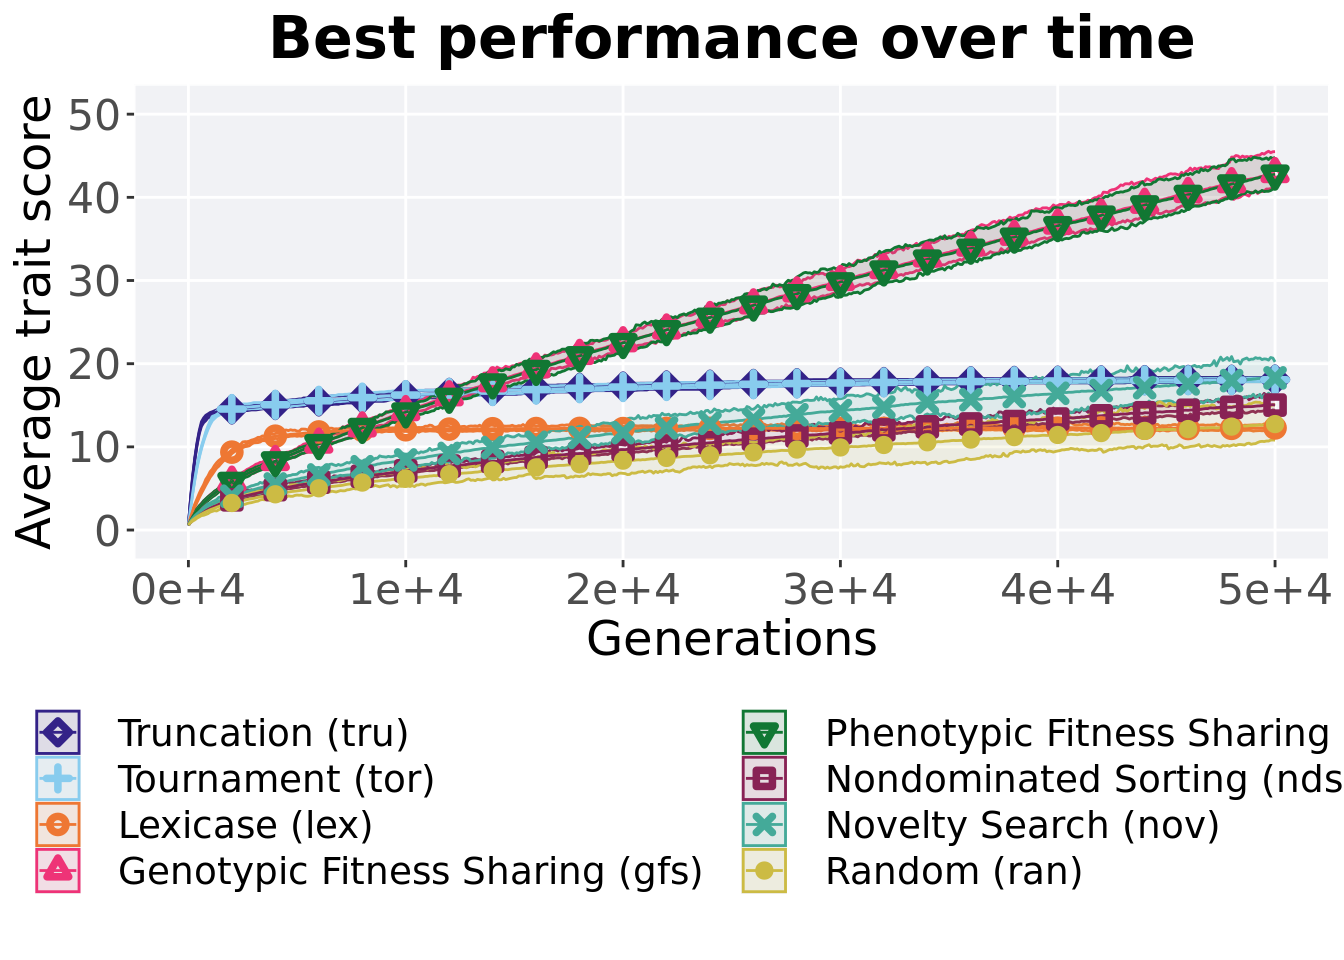
\includegraphics{demo_files/figure-latex/mvc-per-ot-1.pdf}

\hypertarget{best-performance-throughout}{%
\subsection{Best performance throughout}\label{best-performance-throughout}}

Best performance throughout 50,000 generations.

\begin{Shaded}
\begin{Highlighting}[]
\NormalTok{best =}\StringTok{ }\NormalTok{dplyr}\OperatorTok{::}\KeywordTok{filter}\NormalTok{(cc_best, col }\OperatorTok{==}\StringTok{ 'pop_fit_max'} \OperatorTok{&}\StringTok{ }\NormalTok{diagnostic }\OperatorTok{==}\StringTok{ 'multivalley_crossing'}\NormalTok{)}

\CommentTok{# plot = ggplot(best, aes(x = acron, y = val / TRAITS, color = acron, fill = acron, shape = acron)) +}
\CommentTok{#   geom_flat_violin(position = position_nudge(x = .2, y = 0), scale = 'width', alpha = 0.2) +}
\CommentTok{#   geom_point(position = position_jitter(width = .1), size = 1.5, alpha = 1.0) +}
\CommentTok{#   geom_boxplot(color = 'black', width = .2, outlier.shape = NA, alpha = 0.0) +}
\CommentTok{#   scale_y_continuous(}
\CommentTok{#     name="Average trait score",}
\CommentTok{#     limits=c(-1, 51),}
\CommentTok{#     breaks=seq(0,50, 10),}
\CommentTok{#     labels=c("0", "10", "20", "30", "40", "50")}
\CommentTok{#   ) +}
\CommentTok{#   scale_x_discrete(}
\CommentTok{#     name="Scheme"}
\CommentTok{#   )+}
\CommentTok{#   scale_shape_manual(values=SHAPE)+}
\CommentTok{#   scale_colour_manual(values = cb_palette) +}
\CommentTok{#   scale_fill_manual(values = cb_palette) +}
\CommentTok{#   p_theme}

\CommentTok{# plot_grid(}
\CommentTok{#   plot +}
\CommentTok{#     ggtitle("Best performance throughout") +}
\CommentTok{#     theme(legend.position="none"),}
\CommentTok{#   legend,}
\CommentTok{#   nrow=2,}
\CommentTok{#   rel_heights = c(2,.55),}
\CommentTok{#   label_size = TSIZE}
\CommentTok{# )}
\end{Highlighting}
\end{Shaded}

\hypertarget{stats}{%
\subsubsection{Stats}\label{stats}}

Summary statistics for the best performance throughout 50,000 generations.

\begin{Shaded}
\begin{Highlighting}[]
\NormalTok{best}\OperatorTok{$}\NormalTok{acron <-}\StringTok{ }\KeywordTok{factor}\NormalTok{(best}\OperatorTok{$}\NormalTok{acron, }\DataTypeTok{levels =} \KeywordTok{c}\NormalTok{(}\StringTok{'pfs'}\NormalTok{,}\StringTok{'gfs'}\NormalTok{,}\StringTok{'nov'}\NormalTok{,}\StringTok{'tor'}\NormalTok{,}\StringTok{'tru'}\NormalTok{,}\StringTok{'nds'}\NormalTok{,}\StringTok{'ran'}\NormalTok{,}\StringTok{'lex'}\NormalTok{))}
\KeywordTok{group_by}\NormalTok{(best, acron) }\OperatorTok
\StringTok{  }\NormalTok{dplyr}\OperatorTok{::}\KeywordTok{summarise}\NormalTok{(}
    \DataTypeTok{count =} \KeywordTok{n}\NormalTok{(),}
    \DataTypeTok{na_cnt =} \KeywordTok{sum}\NormalTok{(}\KeywordTok{is.na}\NormalTok{(val)),}
    \DataTypeTok{min =} \KeywordTok{min}\NormalTok{(val, }\DataTypeTok{na.rm =} \OtherTok{TRUE}\NormalTok{),}
    \DataTypeTok{median =} \KeywordTok{median}\NormalTok{(val, }\DataTypeTok{na.rm =} \OtherTok{TRUE}\NormalTok{),}
    \DataTypeTok{mean =} \KeywordTok{mean}\NormalTok{(val, }\DataTypeTok{na.rm =} \OtherTok{TRUE}\NormalTok{),}
    \DataTypeTok{max =} \KeywordTok{max}\NormalTok{(val, }\DataTypeTok{na.rm =} \OtherTok{TRUE}\NormalTok{),}
    \DataTypeTok{IQR =} \KeywordTok{IQR}\NormalTok{(val, }\DataTypeTok{na.rm =} \OtherTok{TRUE}\NormalTok{)}
\NormalTok{  )}
\end{Highlighting}
\end{Shaded}

\begin{verbatim}
## # A tibble: 8 x 8
##   acron count na_cnt   min median  mean   max   IQR
##   <fct> <int>  <int> <dbl>  <dbl> <dbl> <dbl> <dbl>
## 1 pfs      50      0 4127.  4288. 4296. 4492. 126. 
## 2 gfs      50      0 4130.  4311. 4310. 4575.  87.6
## 3 nov      50      0 1659.  1883. 1880. 2121. 114. 
## 4 tor      50      0 1784.  1806. 1806. 1827.   9  
## 5 tru      50      0 1784.  1807. 1809. 1835   14.0
## 6 nds      50      0 1463.  1544. 1547. 1656.  54.5
## 7 ran      50      0 1100.  1306. 1314. 1562. 152. 
## 8 lex      50      0 1248.  1273. 1272. 1296.  11.5
\end{verbatim}

Kruskal--Wallis test provides evidence of difference among best performances throughout 50,000 generations.

\begin{Shaded}
\begin{Highlighting}[]
\CommentTok{# kruskal.test(val ~ acron,data = best)}
\end{Highlighting}
\end{Shaded}

Results for post-hoc Wilcoxon rank-sum test with a Bonferroni correction on best performance throughout 50,000 generations.

\begin{Shaded}
\begin{Highlighting}[]
\CommentTok{# pairwise.wilcox.test(x = best$val, g = best$acron, p.adjust.method = "bonferroni",}
\CommentTok{#                      paired = FALSE, conf.int = FALSE, alternative = 'l')}
\end{Highlighting}
\end{Shaded}

\hypertarget{end-of-50000-generations}{%
\subsection{End of 50,000 generations}\label{end-of-50000-generations}}

Best performance in the population at the end of 50,000 generations.

\begin{Shaded}
\begin{Highlighting}[]
\NormalTok{end =}\StringTok{ }\NormalTok{dplyr}\OperatorTok{::}\KeywordTok{filter}\NormalTok{(cc_end, diagnostic }\OperatorTok{==}\StringTok{ 'multivalley_crossing'}\NormalTok{)}
\CommentTok{# plot = ggplot(end, aes(x = acron, y = pop_fit_max / TRAITS, color = acron, fill = acron, shape = acron)) +}
\CommentTok{#   geom_flat_violin(position = position_nudge(x = .2, y = 0), scale = 'width', alpha = 0.2) +}
\CommentTok{#   geom_point(position = position_jitter(width = .1), size = 1.5, alpha = 1.0) +}
\CommentTok{#   geom_boxplot(color = 'black', width = .2, outlier.shape = NA, alpha = 0.0) +}
\CommentTok{#   scale_y_continuous(}
\CommentTok{#     name="Average trait score",}
\CommentTok{#     limits=c(-1, 51),}
\CommentTok{#     breaks=seq(0,50, 10),}
\CommentTok{#     labels=c("0", "10", "20", "30", "40", "50")}
\CommentTok{#   ) +}
\CommentTok{#   scale_x_discrete(}
\CommentTok{#     name="Scheme"}
\CommentTok{#   )+}
\CommentTok{#   scale_shape_manual(values=SHAPE)+}
\CommentTok{#   scale_colour_manual(values = cb_palette) +}
\CommentTok{#   scale_fill_manual(values = cb_palette) +}
\CommentTok{#   p_theme}

\CommentTok{# plot_grid(}
\CommentTok{#   plot +}
\CommentTok{#     ggtitle("Final performance") +}
\CommentTok{#     theme(legend.position="none"),}
\CommentTok{#   legend,}
\CommentTok{#   nrow=2,}
\CommentTok{#   rel_heights = c(2,.55),}
\CommentTok{#   label_size = TSIZE}
\CommentTok{# )}
\end{Highlighting}
\end{Shaded}

\hypertarget{stats-1}{%
\subsubsection{Stats}\label{stats-1}}

Summary statistics for best performance in the population at the end of 50,000 generations.

\begin{Shaded}
\begin{Highlighting}[]
\NormalTok{end}\OperatorTok{$}\NormalTok{acron <-}\StringTok{ }\KeywordTok{factor}\NormalTok{(end}\OperatorTok{$}\NormalTok{acron, }\DataTypeTok{levels =} \KeywordTok{c}\NormalTok{(}\StringTok{'pfs'}\NormalTok{,}\StringTok{'gfs'}\NormalTok{,}\StringTok{'nov'}\NormalTok{,}\StringTok{'tor'}\NormalTok{,}\StringTok{'tru'}\NormalTok{,}\StringTok{'nds'}\NormalTok{,}\StringTok{'ran'}\NormalTok{,}\StringTok{'lex'}\NormalTok{))}
\KeywordTok{group_by}\NormalTok{(end, acron) }\OperatorTok
\StringTok{  }\NormalTok{dplyr}\OperatorTok{::}\KeywordTok{summarise}\NormalTok{(}
    \DataTypeTok{count =} \KeywordTok{n}\NormalTok{(),}
    \DataTypeTok{na_cnt =} \KeywordTok{sum}\NormalTok{(}\KeywordTok{is.na}\NormalTok{(pop_fit_max)),}
    \DataTypeTok{min =} \KeywordTok{min}\NormalTok{(pop_fit_max, }\DataTypeTok{na.rm =} \OtherTok{TRUE}\NormalTok{),}
    \DataTypeTok{median =} \KeywordTok{median}\NormalTok{(pop_fit_max, }\DataTypeTok{na.rm =} \OtherTok{TRUE}\NormalTok{),}
    \DataTypeTok{mean =} \KeywordTok{mean}\NormalTok{(pop_fit_max, }\DataTypeTok{na.rm =} \OtherTok{TRUE}\NormalTok{),}
    \DataTypeTok{max =} \KeywordTok{max}\NormalTok{(pop_fit_max, }\DataTypeTok{na.rm =} \OtherTok{TRUE}\NormalTok{),}
    \DataTypeTok{IQR =} \KeywordTok{IQR}\NormalTok{(pop_fit_max, }\DataTypeTok{na.rm =} \OtherTok{TRUE}\NormalTok{)}
\NormalTok{  )}
\end{Highlighting}
\end{Shaded}

\begin{verbatim}
## # A tibble: 8 x 8
##   acron count na_cnt   min median  mean   max   IQR
##   <fct> <int>  <int> <dbl>  <dbl> <dbl> <dbl> <dbl>
## 1 pfs      50      0 4105.  4272. 4275. 4482. 140. 
## 2 gfs      50      0 4104.  4291. 4290. 4549.  90.7
## 3 nov      50      0 1634.  1825. 1829. 2021. 114. 
## 4 tor      50      0 1784.  1806. 1806. 1827.   9  
## 5 tru      50      0 1784.  1807. 1809. 1835   14.0
## 6 nds      50      0 1440.  1496. 1502. 1644.  42.9
## 7 ran      50      0 1081.  1289. 1274. 1511. 154. 
## 8 lex      50      0 1186.  1229. 1227. 1265.  19.0
\end{verbatim}

Kruskal--Wallis test provides evidence of difference among best performances in the population at the end of 50,000 generations.

\begin{Shaded}
\begin{Highlighting}[]
\CommentTok{# kruskal.test(pop_fit_max ~ acron,data = end)}
\end{Highlighting}
\end{Shaded}

Results for post-hoc Wilcoxon rank-sum test with a Bonferroni correction on best performances in the population at the end of 50,000 generations.

\begin{Shaded}
\begin{Highlighting}[]
\CommentTok{# pairwise.wilcox.test(x = end$pop_fit_max, g = end$acron, p.adjust.method = "bonferroni",}
\CommentTok{#                      paired = FALSE, conf.int = FALSE, alternative = 'l')}
\end{Highlighting}
\end{Shaded}

\bibliography{book.bib,packages.bib}

\end{document}
